% Template LaTeX document for CSSR4Africa Deliverables
% Adapted from documents prepared by EPFL for the RobotCub project
% and subsequently by the University of Skövde for the DREAM project
%
% DV 28/06/2023

\documentclass{CSSRforAfrica}

\usepackage[titletoc,title]{appendix}
\usepackage[colorlinks, urlcolor=blue, linkcolor=black, citecolor=black]{hyperref}
\usepackage{latexsym}
\usepackage{comment}
\usepackage{multirow}
\usepackage{subcaption}
\usepackage[breakable,skins,most]{tcolorbox} % Consolidated tcolorbox options
\usepackage{tabularx,colortbl}
\usepackage[tikz]{bclogo} % for boxes
\usepackage{ragged2e}
\usepackage{dirtree}
\usepackage{listings}
\usepackage{textcomp}
\usepackage{natbib}
\usepackage{url}
\usepackage{graphicx}
\usepackage{array}
\usepackage{longtable}
\usepackage{comment}
\usepackage{algorithm}
\usepackage{algorithmicx}
\usepackage{algpseudocode}

%%% for listing %%%%%%%%%%%%%%%%%%%%%%%%%%%%%%
\captionsetup[figure]{format=hang}
\usepackage{xcolor}
\definecolor{codegreen}{rgb}{0,0.6,0}
\definecolor{codegray}{rgb}{0.5,0.5,0.5}
\definecolor{codepurple}{rgb}{0.58,0,0.82}
\definecolor{backcolour}{rgb}{0.95,0.95,0.92}
\definecolor{greenyellow}{rgb}{0.8, 0.7, 0.10} % Example values, adjust as needed

\lstdefinestyle{withoutNumbering}{
	backgroundcolor=\color{backcolour},   
	commentstyle=\color{codegreen},
	keywordstyle=\color{magenta},
	stringstyle=\color{codepurple},
	basicstyle=\ttfamily\small,
	breakatwhitespace=false,         
	breaklines=true,                 
	captionpos=b,                    
	keepspaces=true,                 
	showspaces=false,                
	showstringspaces=false,
	showtabs=false,                  
	tabsize=2
}
%%%%%%%%%%%%%%%%%%%%%%%%%%%%%%%%%%%%%%%%%%%%%%%%%%%
\definecolor{backcolour}{rgb}{0.95,0.95,0.95}
\definecolor{irongray}{HTML}{6D6E71}
\definecolor{LightGray}{gray}{0.9}

\newcommand{\blank}{~\\}
\newcommand{\checkbox}{{~~~~~~~\leavevmode \put(-7,-1.5){  \huge $\Box$  }}}

\begin{document}
\input{epsf}

%%
%% SHOULD NOT NEED TO BE CHANGED BEFORE THIS POINT
%% ------------------------------------------------
%%


\deliverable{D4.2.3}           
\title{D4.2.3 Sound Detection and Localization}    

\leadpartner{Carnegie Mellon University Africa} % REPLACE with partner name: Carnegie Mellon University Africa or The University of the Witwatersrand
\partner{}                                      

\revision{1.2}            
\deliverabledate{31/12/2023}    
\submissiondate{21/02/2025}   
\revisiondate{16/06/2025}    
\disseminationlevel{PU}
\responsible{Yohannes Haile}      


%%
%% Create the titlepage
%%

\maketitle
 

\section*{Executive Summary}
%===============================================================
\label{executive_summary}
Deliverable D4.2.3 introduces the \texttt{soundDetection} module, a key component designed to detect and localize conspicuous sounds within a robot's hearing range, enabling enhanced interaction and responsiveness of Pepper robot. This module, implemented as a ROS node and it provides two outputs: the direction of arrival (DoA) of the sound, published as an angle in degrees, and a filtered audio signal. Designed to operate reliably in acoustically challenging environments, the module ensures robust performance in real-world conditions. It is integral to the Speech Event (D4.3.2) and Attention Subsytem(D5.3), facilitating Automatic Speech Recognition (ASR) and enabling the robot to focus its attention on sound sources. The deliverable includes a comprehensive documentation package covering the development process, functional specifications, interface design, and testing strategies. A user manual provides clear instructions for building, launching, and configuring the module for use with the Pepper robot. Testing across environments ensures reliability of the soundDetection module.
\newpage
 
\pagebreak
\tableofcontents
\newpage

\section{Introduction}
%===============================================================
The ability to detect and localize sound is fundamental for robots operating in dynamic and interactive environments. Deliverable D4.2.3 addresses this need by developing the soundDetection module, a ROS-based system that identifies conspicuous sounds and determines their direction of arrival (DoA) using interaural time difference (ITD) as the primary localization technique. By leveraging ITD, the module calculates the time delay of sound arrival between microphones, enabling precise auditory localization within the robot’s hearing range. This module enhances the robot’s situational awareness and facilitates more natural human-robot interactions using this auditory cues.

The soundDetection module is critical to enabling higher-level functionalities, such as Automatic Speech Recognition (ASR) and OvertAttention, where auditory input is used to trigger speech processing and direct the robot’s focus toward sound sources. It is designed to work reliably and handle challenging acoustic conditions such as background noise and reverberation.

This deliverable includes the implementation of \texttt{soundDetection} ROS node, which processes multichannel audio signals to output the sound’s direction and the captured audio signal. A configuration file (\texttt{sound\_detection\_configuration.json}) enables flexibility in band-pass filter thresholds, and intensity detection thresholds.

In addition to the software implementation, the deliverable provides a detailed report documenting the module's development process, functional specifications, and testing methodology. A user manual is also included, offering clear guidance on building, configuring, and deploying the module.

\newpage

\section{Requirement Definition}
The \texttt{soundDetection} module is designed to enable robots to detect conspicuous sounds and determine their direction of arrival (DoA) within the hearing range. The key requirements for the module are as follows:

\subsection*{Sound Detection and Localization}
\begin{itemize}
	\item The module must detect conspicuous sounds, such as human voices, and ignore ambient noises or background interference.
	\item Localization must be limited to the azimuth (horizontal) plane and output the DoA as an angle in degrees relative to the robot's Cartesian head frame.
\end{itemize}

\subsection*{Configurable Parameters}
\begin{itemize}
	\item Allow customization through Configuration parameters, such as band-pass filter thresholds, and intensity detection thresholds, must be provided via a (\texttt{sound\_detection\_configuration.json}) file.
\end{itemize}

\subsection*{Input and Output}
\begin{itemize}
	\item \textbf{Input:} Multichannel audio signal from the robot’s microphones.
	\item \textbf{Output:}
	\begin{itemize}
		\item \textbf{Direction of Arrival:} Published on the ROS topic \texttt{soundDetection/direction}.
		\item \textbf{Audio Signal:} Captured left channel audio, published on the ROS \\ topic \texttt{soundDetection/signal}.
	\end{itemize}
\end{itemize}
	
\subsection*{Integration}
\begin{itemize}
	\item Outputs must be compatible with higher-level systems, such as the \texttt{Speech Event} and \\ 
	\texttt{OvertAttention} packages, for Automatic Speech Recognition (ASR) and attention direction.
\end{itemize}

\subsection*{Verbose Mode}
\begin{itemize}
	\item Provide optional diagnostic output in the terminal 
\end{itemize}

\begin{comment}
\subsection{Unit Testing and Validation Requirements}
\begin{enumerate}
	\item Unit Test must be carried out by on Pepper robot using pre-recorded data files as test drivers.
	\item Environmental scenarios such as Air conditioning, chatter, Reverberant rooms, and  Quiet environments for baseline testing must be set up.
	\item Ensure sound detection and localization work under different noise levels and configurations.
	\item Validate outputs for both driver-stub and physical robot tests. 
\end{enumerate}
\end{comment}

\subsection*{Misalignment of the Module}
One of the key misalignment of the \texttt{soundDetection} module is its limited operational range in the azimuth plane. The module can only accurately localize sounds within an angle range of \(-67^\circ\) to \(67^\circ\). This limitation arises due to the smaller distance between the microphones on the robot's head, which affects the cross-correlation technique used for localization. Beyond this range, the cross-correlation results in undefined, reducing the effectiveness of the module in detecting sounds coming from wider angles.

\newpage

\section{Module Specifications}
The sound detection module, implemented as a ROS node named soundDetection, is designed to detect sound within Pepper robot's hearing and provide a filtered audio signal and determine the direction of the sound arrival. 

The input for this module is multi-channel audio from the robot's microphone. For this node we will be primarily be using the FrontLeft and FrontRight microphone to perform localization. For the sound filtering part we will be using just the FrontLeft Microphone.

The output for this module is two topics. The array of audio data will be published on the \texttt{soundDetection/signal} and the direction of conspicuous audio is published on \\ \texttt{soundDetection/direction}.

The module employs a band-pass filtering technique to isolate audio signals within the frequency range typical of human voice. This filtering method effectively attenuates frequencies outside the desired range, ensuring that extraneous sounds are minimized. Additionally, the module utilizes spectral subtraction to remove stationary background noise by analyzing noise profiles during silent intervals. The noise signature identified is then subtracted from the overall audio signal, resulting in a cleaner output. Finally, the refined signal is published for further processing or use in downstream applications.

For the localization, the module utilizes interaural time difference (ITD) to localize sound sources. It employs the Generalized Cross-Correlation with Phase Transform (GCC-PHAT) algorithm to estimate the time delay between signals captured by multiple microphones. This method enhances the accuracy of the delay estimation by emphasizing phase information, which is less susceptible to noise interference. The computed time differences are then used to triangulate the position of the sound source relative to the microphone array. Ultimately, this localization technique enables the pepper robot to orient itself based on the  direction of arrival of the sound.

If verbosemode is set to True in the configuration file, diagnostic messages and the calculated angle of arrival for the conspicuous sound will be printed out. 

A unit test is developed to test the sound detection node under various conditions background noise and background chatter. The tests will be conducted using a driver-stub test platform, which utilizes recorded audio signal from pepper robot stored in the data folder. Additionally, the unit tests can be executed directly on the physical robot to validate real-world performance.

\newpage

\section{Module Design}
\subsection*{Audio Input}
The input for soundDetection ROS node are pepper's microphone located on the top of pepper robot head. Pepper robot has four micophone located on the top of head for this module though we will be using only the two microphone the FrontLeft (\texttt{C}) and FrontRight (\texttt{D)} microphone as on diagram below. The node expects audio to be sampled at 48 kHz and delivered in blocks of 4096 samples. For better sound localization a block of 8192 samples are used for better precision for the sound localization.
The pepper robot has four microphones located at the top of the robot's head as shown in Figure \ref{fig:Microphone}. 
\begin{figure}[!hbpt]
	\centering
	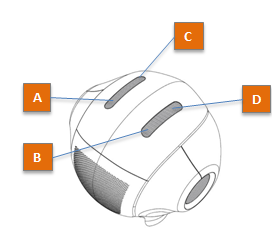
\includegraphics[scale=0.90]{images/Pepper_Microphone.png}
	\caption{Pepper Microphone. Source: \href{http://doc.aldebaran.com/2-5/family/pepper_technical/microphone_pep.html}{Aldebaran}}
	\label{fig:Microphone}
\end{figure}

% create a table to show the Part and Name of the microphone
\begin{longtable}[c]{|p{1.5cm}|p{6cm}|}
	\caption{Pepper Microphone Part and Name.} \label{tab:microphone_part_name}\\
	\hline
	\rowcolor{gray!30}
	\textbf{Part} & \textbf{Name} \\ \hline
	\endhead % header for subsequent pages
	\large{\texttt{A}} & \large{\texttt{MicroRL\_sensor}} \\ \hline
	\large{\texttt{B}} & \large{\texttt{MicroRR\_sensor}} \\ \hline
	\large{\texttt{C}} & \large{\texttt{MicroFL\_sensor}} \\ \hline
	\large{\texttt{D}} & \large{\texttt{MicroFR\_sensor}} \\ \hline
\end{longtable}

\subsection*{Algorithms}
\subsubsection*{WebRTC VAD (Voice Activity Detection)}
The WebRTC Voice Activity Detector (VAD) analyzes short frames of audio, typically 10, 20, or 30 milliseconds, to determine if speech is present. It computes various features such as energy levels, zero-crossing rates, and spectral characteristics for each frame. Based on these features, the VAD compares the computed values against predefined thresholds to decide whether the frame contains speech. It offers multiple aggressiveness modes, ranging from 0 to 3, allowing it to be tuned for different noise environments. In quieter settings, lower aggressiveness modes permit more background noise to be classified as speech, while higher modes are more selective in noisy conditions. The algorithm uses a combination of time-domain and frequency-domain analysis to improve its robustness and accuracy across diverse acoustic scenarios. Ultimately, the VAD outputs a binary decision for each frame, ensuring that sound filtering and localization are only triggered when speech is detected.\cite{webrtcvad}

\subsubsection*{GCC-PHAT}
The GCC-PHAT algorithm is a used method for estimating the time delay between two signals, which is crucial for sound localization. It begins by converting both signals into the frequency domain using the Fourier Transform, allowing for efficient cross-correlation. Then it computes the cross-power spectrum of the two signals and applies a phase transform by normalizing the spectrum with its magnitude, thereby emphasizing phase differences while minimizing amplitude variations. Next an inverse Fourier Transform is applied to the normalized spectrum to obtain a cross-correlation function in the time domain. The algorithm estimates the time delay by locating the peak in this cross-correlation function, which corresponds to the interaural time difference. This delay is then converted into an angle of arrival using the known geometry of the pepper's robot microphone setup(i.e the distance between the two microphone is considered to be (\texttt{0.07m}) and the speed of sound (\texttt{343m/s}) . By focusing on phase information rather than raw amplitude, GCC-PHAT remains robust in noisy or reverberant environments, ensuring accurate estimation of the sound's direction.\cite{knapp1976generalized}

\begin{algorithm}
	\caption{GCC-PHAT Algorithm for Sound Localization}
	\textbf{Require:} Left-channel signal \(x(t)\), right-channel signal \(y(t)\), sampling frequency \(fs\), small constant \(\epsilon\) (to avoid division by zero), and optionally a maximum delay \(T_{max}\)\\
	\textbf{Ensure:} Estimated time delay \(\hat{\tau}\) between \(x(t)\) and \(y(t)\)
	\begin{algorithmic}[1]
		\State Compute the Fourier transform of \(x(t)\): \(X(f) \gets \text{FFT}(x(t))\)
		\State Compute the Fourier transform of \(y(t)\): \(Y(f) \gets \text{FFT}(y(t))\)
		\State Compute the cross-power spectrum: \(R(f) \gets X(f) \cdot Y^*(f)\) \Comment{\(Y^*(f)\) is the complex conjugate of \(Y(f)\)}
		\State Normalize the cross-power spectrum using PHAT:
		\[
		R_{\text{PHAT}}(f) \gets \frac{R(f)}{|R(f)| + \epsilon}
		\]
		\State Compute the inverse Fourier transform to obtain the cross-correlation function:
		\[
		r(\tau) \gets \text{IFFT}(R_{\text{PHAT}}(f))
		\]
		\State Optionally, restrict the search for \(\tau\) to the interval \([-T_{max}, T_{max}]\)
		\State Find the time delay \(\hat{\tau}\) that maximizes \(|r(\tau)|\):
		\[
		\hat{\tau} \gets \arg\max_{\tau} \, |r(\tau)|
		\]
		\State \Return \(\hat{\tau}\)
	\end{algorithmic}
\end{algorithm}

The difference between classical cross correlation and GCC-PHAT is the classical cross correlation computes the similarity between two signals based solely on their amplitudes, which makes it sensitive to variations in signal energy and noise. In contrast, GCC-PHAT introduces a normalization step where the cross-power spectrum is divided by its magnitude, effectively stripping away amplitude information and emphasizing phase differences. This phase emphasis allows GCC-PHAT to be more robust in noisy or reverberant environments, yielding more accurate time delay estimates. By mitigating the influence of amplitude variations, GCC-PHAT can reliably identify the peak corresponding to the true time delay, even when the signals are distorted by noise.

Due to the finite resolution of the audio processing system, the estimated direction of arrival is inherently quantized into a discrete set of values. 
The theoretical position of the maximum cross-correlation value can be calculated by
\[
n = \frac{l \sin \theta}{c} \times F_s,
\]
with our parameters \(l = 0.07\,\text{m}\), \(c = 343\,\text{m/s}\), and \(F_s = 48000\,\text{Hz}\), we first calculate the constant factor:
\[
K = \frac{0.07}{343} \times 48000 \approx 9.795.
\]
Thus, the delay index becomes
\[
n = 9.795 \times \sin \theta.
\]
For unique discrimination, assume that the maximum distinct index is \(n = 9\) (since index values are quantized). Setting
\[
9.795 \times \sin \theta = 9,
\]
we solve for \(\theta\):
\[
\sin \theta = \frac{9}{9.795} \approx 0.9183.
\]
Taking the inverse sine, we obtain:
\[
\theta \approx \arcsin(0.9183) \approx 67^\circ.
\]
Thus, the system can uniquely resolve angles only up to approximately \(67^\circ\) (and \(-67^\circ\) on the negative side) due to the discrete nature of the cross-correlation process. Any angle beyond about \(67^\circ\) will produce the same index, limiting the system's angular resolution unless the sampling frequency or the interaural distance is increased.\\

\subsubsection*{Noise Reduction}
The noisereduce package performs noise reduction by applying spectral gating techniques in the frequency domain. It begins by taking a noisy audio signal and optionally a segment containing only background noise. If no separate noise clip is provided, the function estimates the noise profile from the beginning portion of the signal. The audio is then transformed into a spectrogram using the Short-Time Fourier Transform (STFT), allowing analysis across both time and frequency. From the noise segment, an average noise spectrum is computed, which serves as a reference for identifying and attenuating noise in each time frame. In non-stationary mode, the algorithm adaptively estimates a noise threshold over time and uses a soft sigmoid function to apply a suppression mask that reduces noise while preserving speech components. For stationary noise, a single threshold is used across the entire signal. To minimize artifacts such as choppiness sounds, the mask is smoothed across both frequency and time axes. Finally, the denoised spectrogram is converted back to the time domain using inverse STFT, reconstructing a cleaner audio waveform. \\

\newpage

The diagram below shows how the audio flow chart starting from pepper's microphone until to get filtered audio signal and direction of arrival of the sound.

\begin{figure}[!hbpt]
	\centering
	\includegraphics[scale=0.78]{images/Sound_Diagram.pdf}
	\caption{Sound Detection and Localization Flow Chart}
	\label{fig:Sound_Diagram}
\end{figure}


\newpage

\section{Implementation}
\subsection*{File Organization}
The source code for conducting sound detection and localization is structured into two primary components: \texttt{sound\_detection\_application} and  \texttt{sound\_detection\_implementation}. The \texttt{sound\_detection\_implementation} component encapsulates all the essential functionality required for sound filtering as well as sound localization. Additionally, the sound detection system is equipped with the capability to process various files critical for testing, such as configuration files, input files, and topic files. Meanwhile, the \texttt{sound\_detection\_application} component serves as the entry point, invoking the main functions to run the sound detection node and executing the functions defined within \texttt{sound\_detection\_implementation}.\\

Here is the file structure of the sound detection package:

\begin{figure}[h]	
	\renewcommand*\DTstyle{\ttfamily}
	\dirtree{%
		.1 sound\_detection.
		.2 config.
		.3 sound\_detection\_configuration.json.
		.2 data.
		.3 pepper\_topics.dat.
		.2 launch.
		.3 sound\_detection\_launch\_robot.launch.
		.2 msg.
		.3 sound\_detection\_microphone\_msg\_file.msg.
		.2 src.
		.3 sound\_detection\_application.py.
		.3 sound\_detection\_implementation.py.
		.2 sound\_detection\_requirements.txt.
		.2 README.md.
		.2 CMakeLists.txt.
		.2 package.xml.
	}
	\caption{Updated file structure of the sound detection system}
	\label{fig:sound_detection_directory}
\end{figure}

\subsection*{UML Diagram for the Sound Detection and Localization Module}
The UML diagram provides a clear structural representation of the sound Detection and Localization Module, illustrating the various field and method present in the soundDetectionNode class.

\newpage

Below is the UML diagram of sound\_detection\_implementation.py

\begin{figure}[!hbpt]
	\centering
	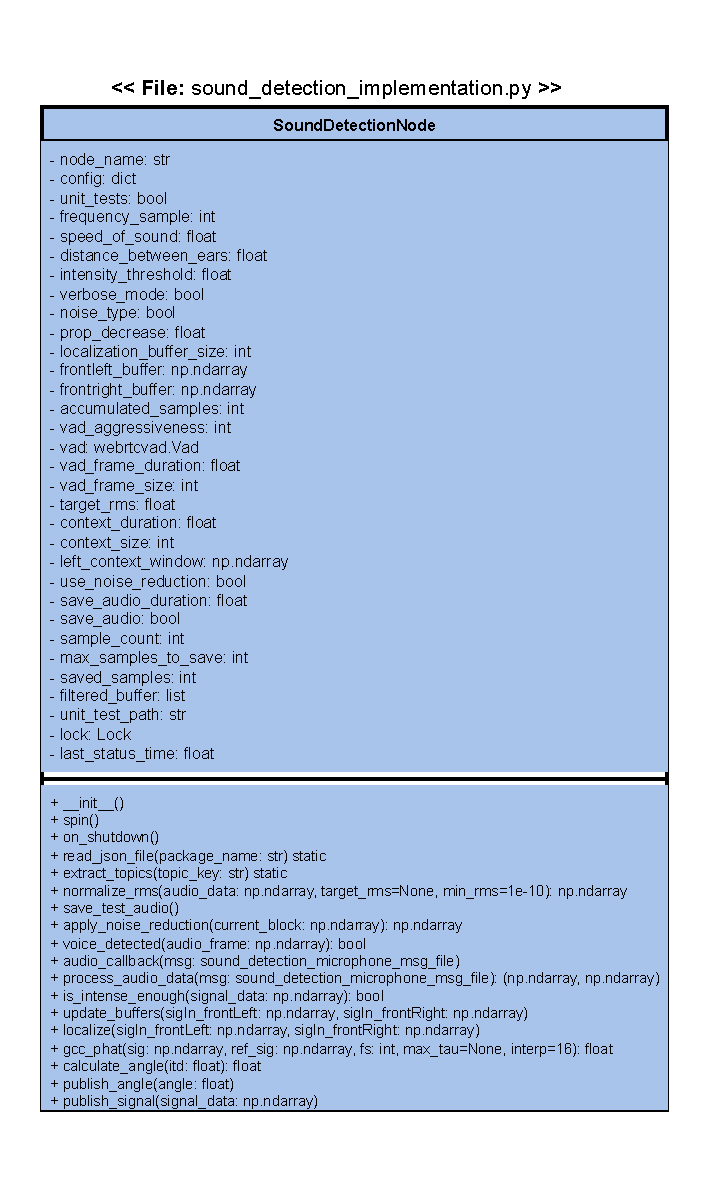
\includegraphics[scale=1.0]{images/Sound_implementation_UML.pdf}
	\caption{Sound detection implementation UML}
	\label{fig:sound_implementation_UML}
\end{figure}

\newpage 


\subsection*{Configuration File}
The operation of the sound detection node is determined by the contents of the configuration file that contains a list of key-value pairs as shown on the table below. 
The configuration file is named \texttt{sound\_detection\_configuration.json}. 


\begin{longtable}{| l | p{10.5cm} |}
	\hline
	\rowcolor{blue!20}
	\textbf{Key} & \textbf{Description} \\
	\hline
	\endfirsthead
	
	\hline
	\rowcolor{blue!20}
	\textbf{Key} & \textbf{Description} \\
	\hline
	\endhead
	
	\texttt{intensityThreshold} & RMS intensity threshold for audio signal detection. Audio frames with RMS values below this threshold are filtered out as background noise. \\
	\hline
	\texttt{distanceBetweenEars} & Physical distance in meters between the left and right microphones, used in GCC-PHAT algorithm for calculating sound source angle from interaural time difference. \\
	\hline
	\texttt{localizationBufferSize} & Buffer size in samples for accumulating audio data before performing sound localization using the GCC-PHAT algorithm. \\
	\hline
	\texttt{vadAggressiveness} & WebRTC Voice Activity Detection aggressiveness level (0-3). Higher values make the VAD more aggressive in filtering out non-speech audio segments. \\
	\hline
	\texttt{contextDuration} & Duration in seconds for the rolling context window used in noise reduction processing. Longer durations provide better noise estimation but increase memory usage. \\
	\hline
	\texttt{useNoiseReduction} & If set to true, applies spectral subtraction noise reduction to the left audio channel using the noisereduce library. \\
	\hline
	\texttt{stationary} & Noise type parameter for the noise reduction algorithm. If true, assumes stationary noise characteristics for more effective filtering. \\
	\hline
	\texttt{propDecrease} & Proportional decrease factor for the noise reduction algorithm. Controls the aggressiveness of noise suppression, with values closer to 1.0 providing more conservative noise reduction. \\
	\hline
	\texttt{verboseMode} & If set to true, enables detailed logging output including RMS normalization details, noise reduction status, and processing diagnostics. \\
	\hline
	
	\caption{Configuration parameters for the sound detection node.}
	\label{tab:sound_detection_config}
\end{longtable}

\subsection*{Input File}
There is no input file the sound detection node.

\subsection*{Output File}
There is no output file the sound detection node. The node display on the terminal direction of the conspicuous sound.

\subsection*{Models}
No models are used for this sound detection node.

\subsection*{Topics File} 
For the test, a selected list of the topics for the robot is stored in the topics file. The topic files are 
written in the .dat file format. The data file is written in key-value pairs where the key is the Microphone  
and the value is the topic. The topics file for the robot is named \texttt{pepper\_topics.dat}.

\subsection*{Launch File}
The launch file \texttt{sound\_detection\_launch\_robot.launch} is designed to initialize pepper sensors based on the specified configuration. It declares several parameters that can be customized to match your network settings.
\begin{itemize}
	\setlength\itemsep{0em}
	\item \texttt{pepper\_robot\_ip}: specifies the IP address of the Pepper robot (default: \texttt{172.29.111.230}).
	\item \texttt{roscore\_ip}: IP address of the ROS master (default: \texttt{127.0.0.1})
	\item \texttt{pepper\_robot\_port}: specifies the communication port for Pepper (default: \texttt{9559}).
	\item \texttt{network\_interface}: specifies the network interface name (default: \texttt{wlp0s20f3}).
	\item \texttt{namespace}: sets the ROS namespace for the naoqi driver (default: \texttt{naoqi\_driver}).
\end{itemize}


\subsection*{Topics Subscribed}
The sound detection node subscribes to the following topics:
\begin{table}[!h]
	\centering
	\begin{tabularx}{\linewidth}{| l | l | X |}
		\hline
		\rowcolor{blue!20} % Light blue background color
		\textbf{Sensor} & \textbf{Topic Name} & \textbf{Message Type} \\
		\hline
		{\footnotesize \texttt{Microphone} }  & {\footnotesize \texttt{/naoqi\_driver/audio}} & {\footnotesize \texttt{sound\_detection\_microphone\_msg\_file}} \\
		\hline
	\end{tabularx}
	\caption{Topics subscribed by the sound detection node.}
\end{table}

\subsection*{Topics Published}

The sound detection node publishes the following topics:
\begin{table}[!h]
	\centering
	\begin{tabularx}{\linewidth}{| l | l | >{\raggedright\arraybackslash}X |}
		\hline
		\rowcolor{blue!20}
		\textbf{Topic Name} & \textbf{Message Type} & \textbf{Description} \\
		\hline
		{\footnotesize \texttt{/soundDetection/signal}}  & {\footnotesize \texttt{std\_msgs/Float32MultiArray}} & {\footnotesize Contains the filtered audio signal corresponding to the input audio block.} \\
		\hline
		{\footnotesize \texttt{/soundDetection/direction}}  & {\footnotesize \texttt{std\_msgs/Float32}} & {\footnotesize Contains the computed angle of arrival (in degrees) of the sound.} \\
		\hline
	\end{tabularx}
	\caption{Topics published by the sound detection node.}
\end{table}

\newpage

\section{Running the Sound Detection Node}
To run the sound detection node, the user must first install the necessary software packages as outlined in 
\href{https://cssr4africa.github.io/deliverables/CSSR4Africa_Deliverable_D3.3.pdf}{Deliverable 3.3}. The required packages
are listed in the {\small\texttt{sound\_detection\_requirements.txt}} file. The user can follow the README file in the sound detection
package to install the required packages. Referring to the implementation section of this deliverable report, the user must 
set the configuration file to the desired parameters. Using the key-value pair, the user can set the intensity threshold, proportional decrease factor for noise reduction, and other parameters. The user can then run the sound detection node by executing the following 
command in the terminal:

\begin{lstlisting}[style=withoutNumbering, language=bash]
	# Launch Pepper robot sensors 
	$ roslaunch cssr_system sound_detection_launch_robot.launch
\end{lstlisting}

\begin{lstlisting}[style=withoutNumbering, language=bash]
	# Run the sound detection node
	$ rosrun cssr_system sound_detection_application.py
\end{lstlisting}

\newpage
\section{Unit Test}
The unit test is designed to validate the sound detection node's functionality under various environment including nose such as background chatter and air conditioning noise  
The test can be performed using a driver-stub test platform, which utilizes recorded audio data stored in the data folder as a rosbag file. The unit test can also 
be executed directly on the physical robot to validate real-world performance. 

The sound detection unit test file structure is as follows: 

\begin{figure}[h]	
	\renewcommand*\DTstyle{\ttfamily}
	\dirtree{%
		.1 unit\_test.
		.2 sound\_detection\_test.
		.3 config.
		.4 sound\_detection\_test\_configuration.json.
		.3 data.
		.4 sound\_detection\_test\_input\_sound\_distance.bag.
		.4 sound\_detection\_test\_input\_sound\_angle.bag.
		.4 sound\_detection\_test\_input\_sound\_noise.bag.
		.4 sound\_detection\_test\_unfiltered\_\{timestamp\}.wav.
		.4 sound\_detection\_test\_speech\_filtered\_\{timestamp\}.wav.
		.4 sound\_detection\_test\_direction\_data\_\{timestamp\}.txt.
		.3 launch.
		.4 sound\_detection\_launch\_robot.launch.
		.4 sound\_detection\_launch\_test\_harness.launch.
		.3 src.
		.4 sound\_detection\_test\_application.py.
		.4 sound\_detection\_test\_implementation.py.
		.3 CMakeLists.txt.
		.3 Package.xml.
		.3 README.md.
	}
	\caption{File structure of the sound detection unit test.}
	\label{fig:sound_detection_unit_test}
\end{figure}

The test cases for the sound detection node that are going to be evaluated are as follows:

\begin{longtable}{| l | p{13cm} |}
	\hline
	\rowcolor{blue!20}
	\textbf{Test Case} & \textbf{Description} \\
	\hline
	\endfirsthead
	
	\hline
	\rowcolor{blue!20}
	\textbf{Test Case} & \textbf{Description} \\
	\hline
	\endhead
	
	\text{Sound Distance} & Verifies the sound detection node's capability to accurately measure the distance of a sound source. This bag file contains audio recordings with variations in source-to-microphone distance, allowing evaluation of distance estimation performance. \\
	\hline
	\text{Sound Angle} & Evaluates the system's ability to compute the angle of arrival of the sound. The bag file includes audio samples recorded from different azimuth angles to validate the accuracy of the GCC-PHAT based localization. \\
	\hline
	\text{Sound Noise} & Assesses the robustness of the sound detection node under noisy conditions. This bag file features audio with various levels of background noise, testing the effectiveness of filtering and voice activity detection (VAD) algorithms. \\
	\hline
	\caption{Test cases for sound detection node evaluation using specific bag files.}
	\label{tab:sound_detection_tests}
\end{longtable}


\noindent \textbf{Note:} Valid values for \texttt{bag\_file} include: \texttt{sound\_distance}, \texttt{sound\_angle}, \texttt{sound\_noise}.

\newpage

Below is the UML diagram of sound\_detection\_test\_implementation.py

\begin{figure}[!hbpt]
	\centering
	\includegraphics[scale=1.0]{images/Sound_detection_test_implementation.pdf}
	\caption{Sound detection implementation test UML}
	\label{fig:sound_implementation_test_UML}
\end{figure}

\subsection*{Configuration File}
The configuration file for the sound detection unit test is named \\
\texttt{sound\_detection\_test\_configuration.json} and contains the following key-value pairs:

\begin{longtable}{| l | p{10.5cm} |}
	\hline
	\rowcolor{blue!20}
	\textbf{Key} & \textbf{Description} \\
	\hline
	\endfirsthead
	
	\hline
	\rowcolor{blue!20}
	\textbf{Key} & \textbf{Description} \\
	\hline
	\endhead
	
	\texttt{recordFiltered} & If set to true, records and saves the filtered audio signal. \\
	\hline
	\texttt{recordUnfiltered} & If set to true, records and saves the raw audio signal before processing. \\
	\hline
	\texttt{recordDuration} & Duration in seconds for which audio is recorded. \\
	\hline
	\texttt{saveDirectionData} & If set to true, saves calculated direction-of-arrival data for later analysis. \\
	\hline
	\texttt{targetRMS} & Target root-mean-square (RMS) level for audio normalization. \\
	\hline
	\texttt{applyNormalization} & If true, applies normalization to the audio signal based on targetRMS. \\
	\hline
	\texttt{verboseMode} & If set to true, prints debug information and logs to help with diagnostics and testing. \\
	\hline
	
	\caption{Configuration parameters for the sound detection test node.}
	\label{tab:sound_detection_test_config}
\end{longtable}

\subsection*{Launch File}
The launch file \texttt{sound\_detection\_test\_launch\_robot.launch} is designed to support testing the sound detection node with a live audio input from Pepper's microphone or a recorded a rosbag audio. It provides several configurable arguments to customize the test environment.   

The launch file has the following parameter that can be passed.

\begin{longtable}{| l | p{11cm} |}
	\hline
	\rowcolor{blue!20}
	\textbf{Parameter} & \textbf{Description} \\
	\hline
	\endfirsthead
	
	\hline
	\rowcolor{blue!20}
	\textbf{Parameter} & \textbf{Description} \\
	\hline
	\endhead
	
	\texttt{robot\_ip} & IP address of the robot for establishing network connection (default: 172.29.111.230) \\
	\hline
	\texttt{roscore\_ip} & IP address of the ROS master node for distributed system communication (default: 127.0.0.1 for localhost) \\
	\hline
	\texttt{robot\_port} & Port number used for robot communication and data exchange (default: 9559) \\
	\hline
	\texttt{network\_interface} & Specific network interface identifier for network communication (default: wlp0s20f3) \\
	\hline
	\texttt{namespace} & ROS namespace for organizing and isolating naoqi driver nodes and topics (default: naoqi\_driver) \\
	\hline
	\texttt{audio\_file} & Specifies the audio file selection for playback during testing (default: sound\_distance) \\
	\hline
	\texttt{use\_recorded\_audio} & Boolean flag to enable pre-recorded audio playback instead of live microphone input (default: true) \\
	\hline
	\caption{Launch file parameters and their descriptions.}
	\label{tab:launch_parameters}
\end{longtable}

This setup allows flexible testing of the sound detection node using live or recorded audio data sources with consistent parameters across different hardware.\\
The launch file \texttt{sound\_detection\_test\_launch\_test\_harness.launch} launches the \\ \texttt{sound\_detection }node and \texttt{sound\_detection\_test} node that runs the unit test based on configuration file in the \texttt{sound\_detection\_test}.

\subsection*{Topics Subscribed}
The sound detection test node subscribes to the following topics:
\begin{table}[!h]
	\centering
	{\fontsize{9.0}{12.0}\selectfont % <- apply inside the table
		\begin{tabularx}{\linewidth}{| l | l | X |}
			\hline
			\rowcolor{blue!20}
			\textbf{Audio Source} & \textbf{Topic Name} & \textbf{Message Type} \\
			\hline
			\texttt{PepperMicrophone} & \texttt{/naoqi\_driver/audio} & \texttt{sound\_detection\_microphone\_msg\_file} \\
			\hline
		\end{tabularx}
	}
	\caption{Topics subscribed by the sound detection test node.}
\end{table}


In addition it publishes to \texttt{/soundDetection/signal} for processed audio data and \\
 \texttt{/soundDetection/direction} for calculated sound source angles.

\subsection*{Running Sound Detection and Localization Unit Test}
The user can execute the following commands in the terminal to run the unit test for sound detection node.
\begin{lstlisting}[style=withoutNumbering, language=bash]
	# Launch unit test with live audio from Pepper robot
	$ roslaunch unit_tests sound_detection_test_launch_robot.launch use_recorded_audio:=false
	# or
	# Launch unit test with recorded audio file
	$ roslaunch unit_tests sound_detection_test_launch_robot.launch use_recorded_audio:=true audio_file:=sound_distance
	
\end{lstlisting}
\begin{lstlisting}[style=withoutNumbering, language=bash]
	# Activate the virtual environment:
	source cssr4africa_sound_detection_env/bin/activate
\end{lstlisting}
\begin{lstlisting}[style=withoutNumbering, language=bash]
	# Run the sound detection node with custom robot IP and port
	$ roslaunch unit_tests sound_detection_test_launch_robot.launch
\end{lstlisting}

The unit test will automatically save filtered audio samples to the data directory validation of the noise reduction and voice activity detection algorithms.

\newpage
\bibliographystyle{unsrt}
%================================================================
\bibliography{cognitive_systems.bib}                                     % REPLACE with correct filename
\addcontentsline{toc}{section}{References}

\pagebreak
\section*{Principal Contributors}
%===============================================================
\label{contributors}
\addcontentsline{toc}{section}{Principal Contributors}
The main authors of this deliverable are as follows (in alphabetical order).
\blank
~
\blank
Yohannes Haile, Carnegie Mellon University Africa.\\    % REPLACE with correct name and affiliation
David Vernon, Carnegie Mellon University Africa. \\                                                                           % REMOVE
 

  
\newpage
\section*{Document History}
%================================================================
\addcontentsline{toc}{section}{Document History}
\label{document_history}

\begin{description}

\item [Version 1.0]~\\
First draft. \\
Yohannes Haile. \\        
26 February 2025   

\item [Version 1.1]~\\
Renamed \texttt{soundDetectionConfiguration} to \texttt{sound\_detection\_configuration}. \\
Updated configuration parameters by adding new parameters and detailed description .\\
Replaced separate band-pass filtering and spectral subtraction sections with unified noise reduction implementation using noisereduce package.\\
Changed from underscore to space separation in test file names.\\
Expanded UML diagrams with detailed class attributes, methods, and added test implementation UML.\\
Updated test file naming convention, changed from single MP3 output to multiple timestamped WAV/TXT files, and redesigned test configuration parameters.\\
Added launch file parameters including support for both live and recorded audio testing.\\
Yohannes Haile. \\
23 May 2025                                          

\item [Version 1.2]~\\
Fixed typos. \\
David Vernon. \\       
16 June 2025   


\end{description}

\end{document}

